% book.tex -- Copyright (c) 2004, Brian C. Ladd
%
%  Author : Brian C. Ladd 
%  Created: Wed Jul 07 12:03:49 2004 by blad
%  Revised: Fri Dec 28 15:27:43 2007 by blad
%  
\def\FileCreated{Wed Jul 07 12:03:49 2004}
\def\FileRevised{Fri Dec 28 15:27:43 2007}
\documentclass[12pt,oneside]{memoir}
\usepackage{epsfig}
\usepackage{graphicx}
\usepackage[usenames]{color}
\usepackage{xltxtra}
\usepackage{fontspec}
\usepackage{textcomp}
\usepackage{pstricks}
\usepackage{listings}[2000/08/23] 

\usepackage{rotating}
\usepackage{exercise}
% ----- Fonts -----
\defaultfontfeatures{Scale=MatchLowercase,Mapping=tex-text}
\setmainfont{Gentium Book Basic}
\setmonofont{Bitstream Vera Sans Mono}
\setsansfont{Arial}
% ----- Fonts -----

\definecolor{nicered}{rgb}{.647,.129,.149}
\definecolor{listinggray}{gray}{0.1}
\definecolor{templategrey}{gray}{0.85}
\definecolor{NewtonsApple}{gray}{.95}
\definecolor{commandlinebackground}{gray}{.90}
\definecolor{commandlineforeground}{gray}{0.20,}
\definecolor{commandpromptforeground}{gray}{0.55}

\newcommand\code[1]{\lstinline^#1^}
\newcommand\fname[1]{\texttt{#1}}
\newcommand\note[1]{\unskip\footnote{#1}}
\newcommand\foreign[1]{\emph{#1}}
\newcommand\ensurecomma{%
  \@ifnextchar,{}{\@latex@error{Don’t forget the comma!}{}}}
\newcommand\eg{\foreign{e.g.}\ensurecomma}
\newcommand\ie{\foreign{i.e.}\ensurecomma}
\newcommand\cf{\foreign{cf.\@}}

\newcommand\ensuresingleperiod{\@ifnextchar.{}{.\@}}
\newcommand\etc{\foreign{etc}\ensuresingleperiod}
\newcommand\etal{\foreign{et al}\ensuresingleperiod}

\DeclareGraphicsExtensions{.eps,.pdf,.png,.gif,.jpg}

\newcounter{LabPhase}
\setcounter{LabPhase}{0}%

\newenvironment{LabExercises}{%
\renewcommand{\ExerciseListName}{Question}%
\renewcommand{\ExerciseListHeader}{\textbf{%
   Phase\ExerciseHeaderNB. }}
\begin{ExerciseList}}%
{\end{ExerciseList}}
\newcommand{\LabExercise}{\Exercise[name={Lab Phase\ExerciseHeaderNB},counter={LabPhase}]}
\newcounter{CheckPoint}
\setcounter{CheckPoint}{1}%

\newcommand{\Checkpoint}{\textbf{Checkpoint \theCheckPoint }:: \addtocounter{CheckPoint}{1}}


\lstset{language=java,
  basicstyle=\small\ttfamily,
  numbers=none, 
  numberstyle=\tiny, 
  stepnumber=1, 
  numbersep=5pt,
  frame=single,
  captionpos=b,
  rulecolor=\color{nicered}
}

\lstdefinelanguage{cline}
{
  morecomment=[s][\color{commandpromptforeground}]{ }{ },
} 

\lstnewenvironment{commandline}[1][]
  {\lstset{language=cline,numbers=none,frame=none,backgroundcolor=\color{commandlinebackground},basicstyle=\color{commandlineforeground},nolol,#1}}
  {}

\setlength{\hoffset}{0in}
\setlength{\voffset}{0in}
\settypeblocksize{9.5in}{7.5in}{*}
\setlrmargins{0.5in}{*}{1}
\setulmargins{0.75in}{*}{*}
\setheadfoot{\onelineskip}{2\onelineskip}
\checkandfixthelayout

\begin{document}

\begin{center}
\Large{CIS 201 Fall 2008: Lab 8\\Tic Tac Toe}
\end{center}

\begin{itemize}
\item Implementing a class revisited.
\item Using \code{ArrayList}
\item Game components with ``state''
\end{itemize}

\begin{figure}[htb]
  \begin{center}    
    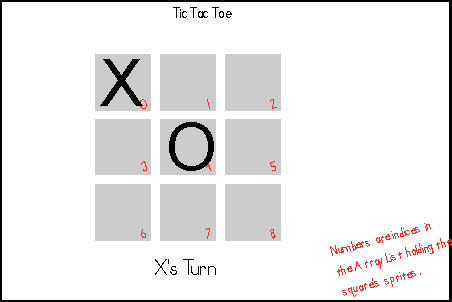
\includegraphics[width=5in]{Drawings/ticTacToe-design}  
    \caption{TicTacToe Design}
  \label{fig:design}
  \end{center}
\end{figure}

\begin{LabExercises}
\LabExercise Consider a simple version of Tic Tac Toe: your
\code{Game} creates and positions nine sprites on the screen. Then, in
\code{advance} you would check for mouse clicks, comparing any click
to each of the sprites. If one is clicked \emph{and} it is empty,
update the sprite with the current player's symbol and change who's
turn it is. Make sure to check for winning and draws somewhere.

Think about how \code{advance} would look. Assuming the sprites are in
an \code{ArrayList}, there would be a big loop with many nested
\code{if} statements in it. This code is too complex to hold in your
mind, all at once.

How do computer programmers respond to complexity? 

\emph{Abstraction!}

Abstraction is the hiding of details of some rule or some
component. It can be applied by writing methods with descriptive names
that make it easier to express the solution at a higher
level. Abstraction can also be applied by breaking responsibility for
the solution across multiple components. The ``simple'' approach given
above is difficult because the Tic Tac Toe game is responsible for
handling both game-level details \emph{and} square-level
details. A separation of responsibility is possible if we build
``smart'' squares; this is a standard technique in object-oriented
design, the creation of objects that ``know what to do''.

Before reading on, you and your partner should pull out a piece of
paper and write down what activities a Tic Tac Toe game must
support. Divide up your list into game-level and move-level
activities. 

\Checkpoint Show your list of activities to one of the lab instructors
before proceeding. This is very important. You will also type your
list into the header comments of your game.
\newpage
When designing this lab, the following responsibilities seemed necessary.
Each square is responsible for:
\begin{itemize}
\item Advancing the state of the square (each frame):
  \begin{itemize}
  \item Checking whether it is legal to click on the square (it is not
    legal if the square is not empty)
  \item Checking whether it has been clicked
  \item If it has been clicked, updating according to which player's
    turn it was and ending the turn.
  \end{itemize}
\item \code{isEmpty} to determine whether or not the square is occupied.
\item Return the current state of the square (``X'', ``O'', or `` '').
\end{itemize}

The game is then responsible for
\begin{itemize}
\item Setting up the game: creating the squares, scaling and
  positioning them.
\item Advancing every square every frame.
\item Showing status.
\item Returning the current player (``X'', ``O'').
\item Ending a turn.
  \begin{itemize}
  \item Checking if the current player has won.
  \item Checking if there is a cat's game.
  \item Otherwise, change which player's turn it is.
  \end{itemize}
\end{itemize}

This lab builds two cooperating classes, \code{TicTacToe} and
\code{TicTacToeSquare}, each fulfilling one of these sets of
requirements.

Note \emph{how} the two classes cooperate: \code{TicTacToe} will need
references to all of the squares so that it can call \code{advance}
for each of them; \code{TicTacToeSquare} needs a reference to the game
of which it is a part to be able to check for mouse clicks, determine
whose turn it is, and to be able to end a turn. This means that, like
the \code{OneDie} class, squares will be constructed with a reference
to their game.

\LabExercise Start the \code{TicTacToe} and \code{TicTacToeSquare}
classes. One should extend \code{Game}, the other should extend
\code{CompositeSprite}. As we have discussed in class, we will build
this lab one piece at a time; that means we will first get the squares
to draw in the right places. Then we will make them aware of mouse
clicks, and then, finally, we will make the game check for end-of-game
conditions. 

\code{TicTacToeSquare} should create a rectangle sprite of a dark
(non-black) color. You will add the ``X'' and ``O'' sprite later. This
means writing a \emph{constructor} for the class; there is no need for
anything else right now.

What \emph{parameters} does the constructor require? Since a
\code{Game} is required for getting colors (and, eventually, checking
for mouse clicks), you should pass in the game when constructing a
square. You will have a field in \code{TicTacToeSquare} to refer to
the game; perhaps something like this:

\begin{lstlisting}
  private Game theGame;
\end{lstlisting}

Then you will call the constructor with something like this (in
\code{TicTacToeSquare}). 

\begin{lstlisting}
  TicTacToeSquare someSquare = new TicTacToeSquare(this);
\end{lstlisting}

The reference to the \code{Game} makes it possible to check who's
turn it is and get mouse clicks.

\code{TicTacToe} should construct nine \code{TicTacToeSquare} objects
and put them in an \code{ArrayList}. They should be distributed in a 3
x 3 grid against the top of the screen. Each should be 0.20 screens
square, centers of rows and columns should be 0.25 apart (at 0.25,
0.50, and 0.75 for the columns, at 0.10, 0.35, and 0.60 for the rows).

How the heck should we go from an index into an \code{ArrayList} to
its corresponding screen coordinates? You should create two methods
for \code{TicTacToe}, \code{row} and \code{column}, each of which
takes a single integer parameter, the index into the \code{ArrayList}
and then returns the row (or column) where that element belongs (0, 1,
or 2). Then you can use a simple linear equation to go from column
number to screen coordinates (and the same for rows).

You should also set up an integer to keep track of which player's turn
it is (0 for ``X'', 1 for ``O''), a \code{StringSprite} to hold a
status message (scale to 0.10, position at the bottom-center of screen
at 0.9 down (the reason the board is so high)).

\Checkpoint When you have the nine dark boxes on the screen, raise
your hand and signal one of the lab instructors to come and look at
your code. Expect to be asked to show/explain your \code{row} and
\code{column} methods.

\LabExercise Create methods to update the status message. You will
need to be able to tell the user who's turn it is, who won, and that
the game is a draw. Also, in the game ending messages, tell the user
to press the space bar to play again. Modify your \code{setup} program
so that it displays which player's turn it is.

\LabExercise \code{TicTacToeSquare} needs to track its own
contents. This means you need a \code{content} field (which should
match the type of the turn tracker in the game). Initialize the
content to -1 (to indicate empty). 

Implement \code{isEmpty} (a public, Boolean method) and a getter
method for the content (so \code{TicTacToe} can see the contents; why
does the game need that information?).

To display the content, add a \code{StringSprite} field. Scale should
be 1.0 and it should initially contain the empty string. Set its color
to some light color and make sure the sprite is added to the
composite. When you set the content of your square, you will set the
text to either ``O'' or ``X''.


\LabExercise Create an \code{advance} method in \code{TicTacToeSquare}
and call it from \code{TicTacToe}'s \code{advance}.

Declare a new method for \code{TicTacToeSquare} called \code{advance};
model it on the \code{advance} in the game. Inside the method do the
following:

\begin{lstlisting}
  if ((this square is empty) && (the mouse has been clicked)) 
    if (this sprite intersects mouse click)
      update content
      update appearance of StringSprite
      call theGame.finishTurn
\end{lstlisting}

In \code{TicTacToe}, call the \code{advance} method for every square
on every frame. If you have to do something with every element in an
\code{ArrayList}, what should you be thinking?

You can comment out the call to \code{finishTurn}; that should permit
you to compile your program and click on the various squares and make
them all ``X'' (turn doesn't change yet). Remember, incremental
development, getting a little bit working before moving on, is another
way to control complexity.

\LabExercise Implement \code{TicTacToe.finishTurn}: it takes no
parameters and just changes who's turn it is. If turn was 0, make it 1
and if it was 1, make it 0.

\Checkpoint Show one of the lab instructors your current program. It
should be possible to click on each of the empty squares and turn it
to an ``X'' or an ``O''. 

\LabExercise Add checking for winning board position and cat's
game. You should modify \code{finishTurn} to something like the
following:

\begin{lstlisting}
  if (winner(turn)) {
    // handle win
  } else if (catsGame()) {
    // handle cat's 
  } else {
    // change who's turn it is as before
  }
\end{lstlisting}

Now you have to write the two methods listed. How will you check if it
is a cat's game? Given that squares can give you their content it
should be easy to check whether or not there are any empty squares:
call \code{isEmpty} in \code{catsGame} for every square in the
game...every square in the \code{ArrayList}...what should you be
thinking? 

The \code{winner} method is a touch messier: check the eight different
ways that a game can be won. The player who just moved is provided as
a parameter to the method so you can just check for contents matching
that value.

To make the logic easier to follow, you might want a method, say
\code{ndx} which, given a row and a column, returns the index in the
\code{ArrayList} corresponding to that element. That means that
checking one of the diagonals would just be:

\begin{lstlisting}
    (board.get(ndx(0, 0)).getContent() == turn &&
     board.get(ndx(1, 1)).getContent() == turn &&
     board.get(ndx(2, 2)).getContent() == turn)
\end{lstlisting}

\noindent
This Boolean expression will be true if and only if the values on the
main diagonal equal the turn variable. So long as \code{turn} is
either 0 or 1, we will only return true for a win along that diagonal.

\Checkpoint Flag down a lab instructor and show them that your game
detects a cat's game and a win. 

\LabExercise Finally, set up so the game can start over. Add a flag,
\code{waiting} which is set to \code{false} in \code{setup}. Then, in
\code{advance}, if \code{waiting} is \code{true}, check for the
player pressing the space bar. If they do, call \code{startOver()} to
restart the game. 

Where would \code{waiting} be set? How about in the three-way
\code{if} where you check for winning and cat's games. If it is a win
(or a cat's game), then the game is waiting to start over so you set
the flag. That way the space bar doesn't reset the game until the
current game is over. 

\LabExercise Upload Your Java files.

Make sure both authors' names are in all of the header comments!

Type the two lists of features (from check point 1) into the header
comment of \code{TicTacToe}. Clearly label them as to which are square
and which are game responsibilities.

Go to Moodle; you will find an assignment in week 9 labeled
\textbf{Lab8}. Go there and upload all of the Java files you
created/modified in lab today. Note that there will be other files in
your \fname{Lab8} directory. You want to make sure you upload just the
\fname{.java} file.

Also make sure that both partners have copies of the program. This
program has some bearing on the current assignment so you probably
want to have this code around. Comments will also be very helpful in
this program for exactly that reason.

\end{LabExercises}


\end{document}

%%% Local Variables: 
%%% mode: latex
%%% End: 

% LocalWords:  Moodle Ladd's login emacs
